\section{Remote Logging}
\subsection{Problem}
\begin{frame}[plain]
	\frametitle{Remote Logging}
	\framesubtitle{Problem}
	\begin{center}
		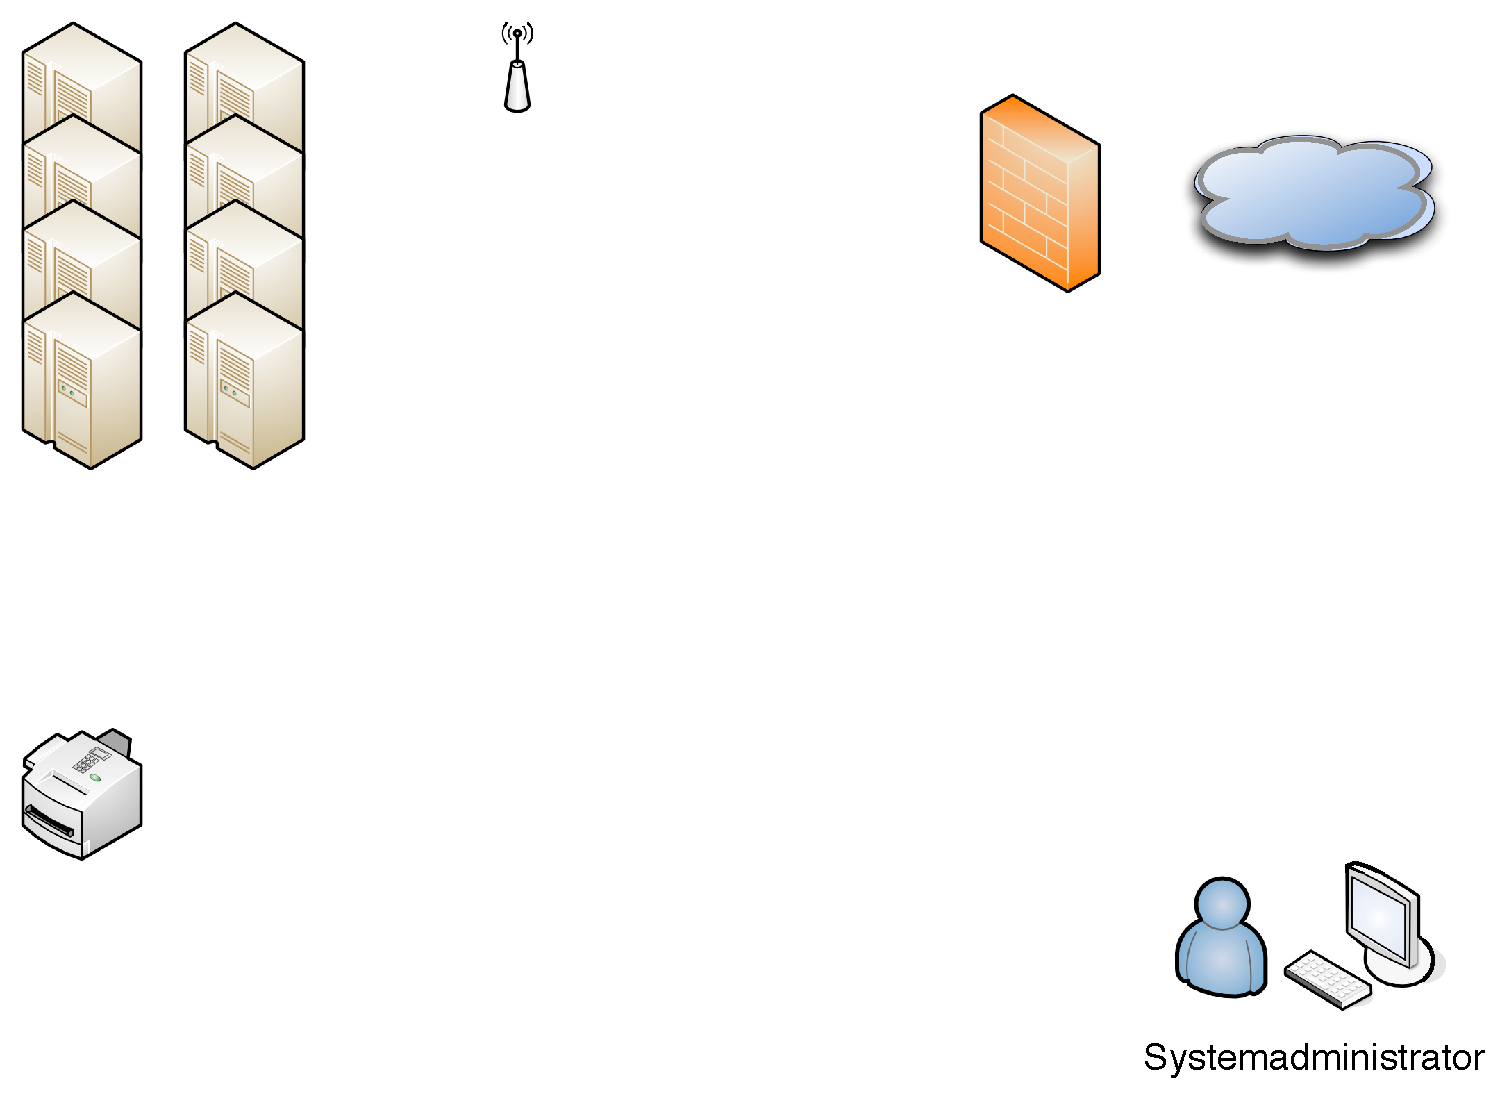
\includegraphics[width=\linewidth]{images/remote_logging_01.eps}
	\end{center}
\end{frame}

\subsection{Panic}
\begin{frame}[plain]
	\frametitle{Remote Logging}
	\framesubtitle{Panic}
	\begin{center}
		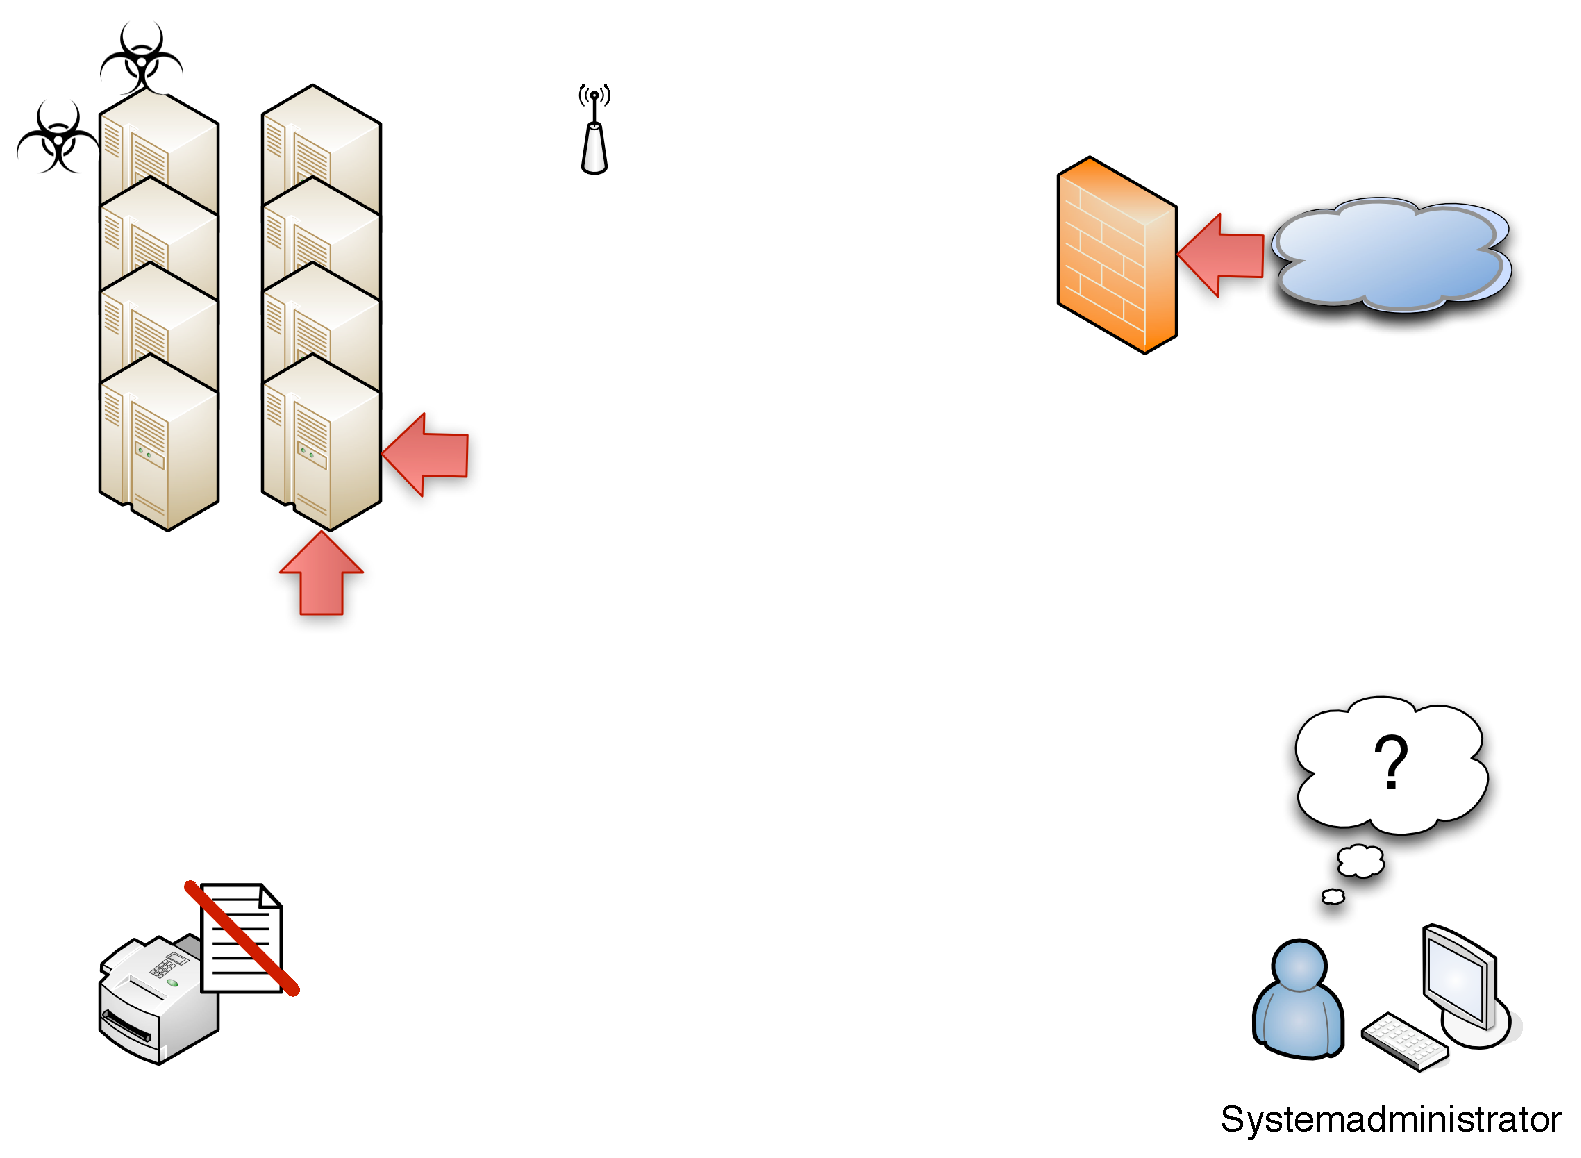
\includegraphics[width=\linewidth]{images/remote_logging_02.eps}
	\end{center}
\end{frame}

\subsection{Don't Panic}
\begin{frame}[plain]
	\frametitle{Remote Logging}
	\framesubtitle{Don't Panic}
	\begin{center}
		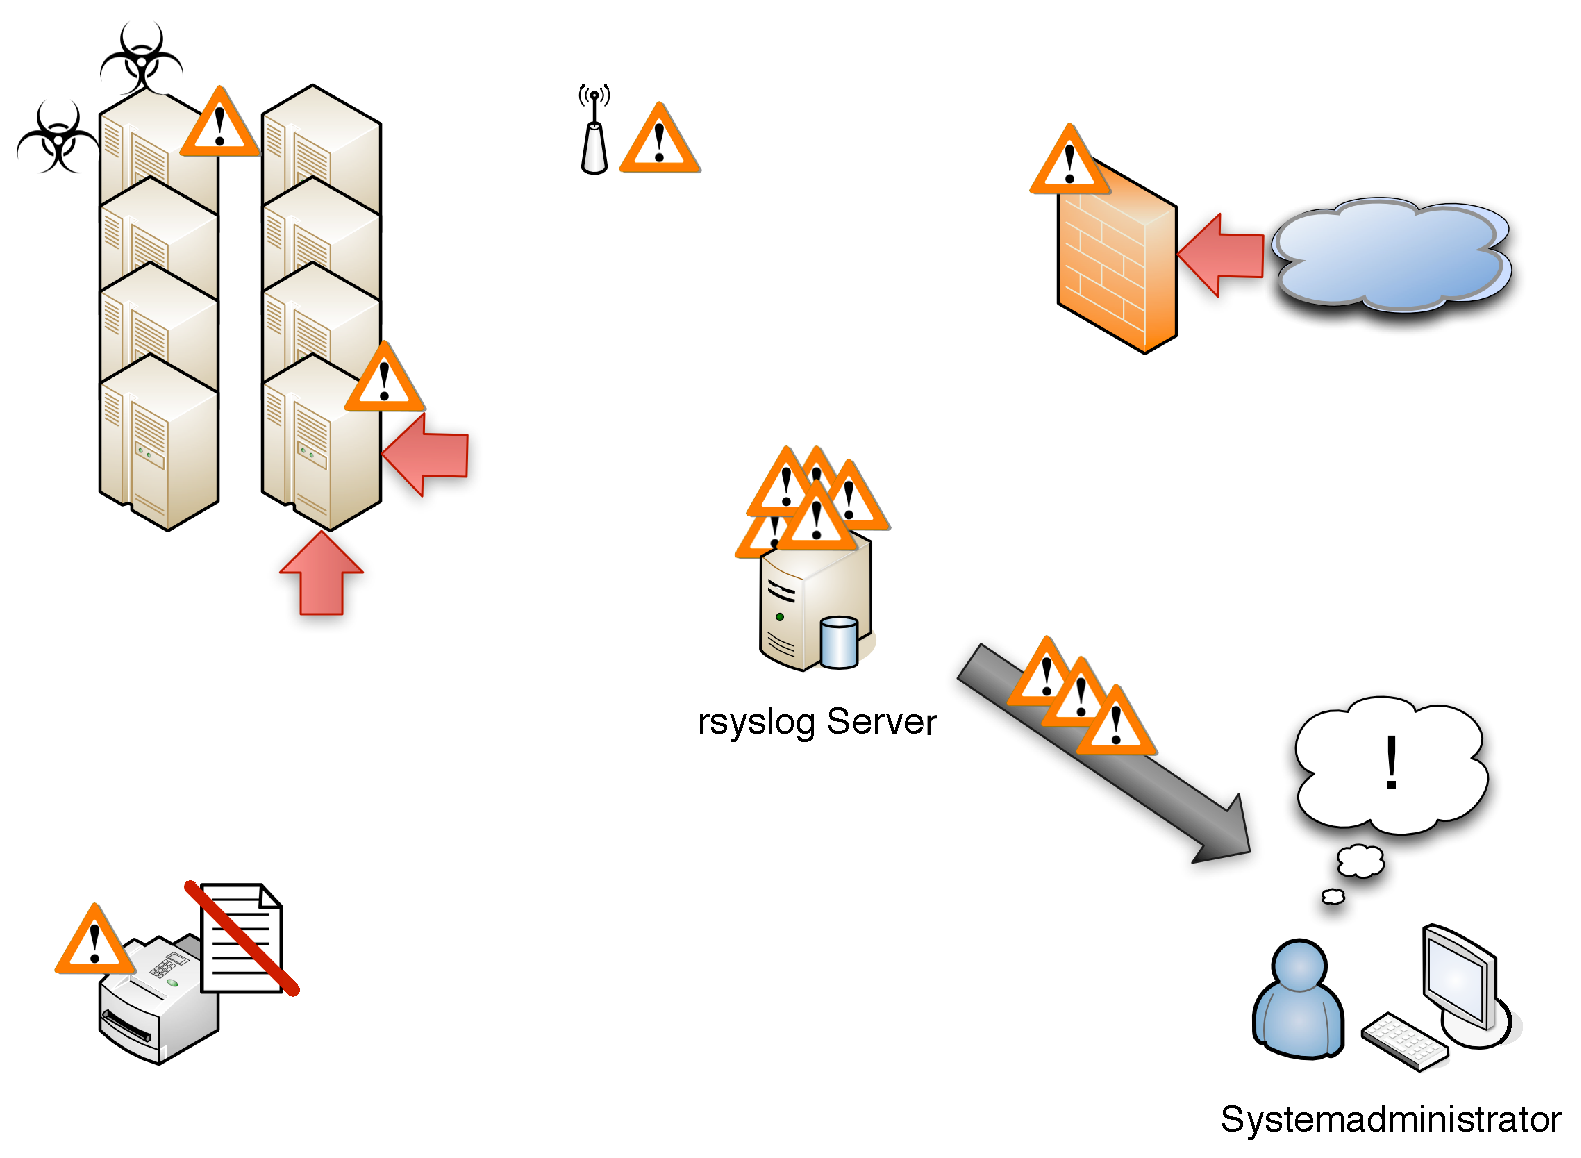
\includegraphics[width=\linewidth]{images/remote_logging_03.eps}
	\end{center}
\end{frame}

\subsection{Ziele}
\begin{frame}
	\frametitle{Remote Logging}
	\framesubtitle{Ziele}
	\begin{itemize}
		\item Alle Informationen an einem zentralen System
		\item Archivierung ist zentralisiert
		\item Alarmierung
		\item Monitoring
	\end{itemize}
\end{frame}